%!TEX program = xelatex
% Note: this template must be compiled with XeLaTeX rather than PDFLaTeX
% due to the custom fonts used. The line above should ensure this happens
% automatically, but if it doesn't, your LaTeX editor should have a simple toggle
% to switch to using XeLaTeX.

\documentclass[
  aspectratio=169, % Uncomment to use an aspect ratio of 16:9 (160 mm by 90 mm)
  %aspectratio=43, % Uncomment to use an aspect ratio of 4:3 (128mm by 96mm)
  t, % Top align all slide content by default
  onlytextwidth, % Typeset content in columns at text width
  10pt, % Default font size, use 10pt for the 16:9 aspect ratio and 8pt for the 4:3 aspect ratio
]{beamer}

\usepackage{../../ImperialTheme/beamer/beamerthemeImperial} % Use the Imperial theme
\usepackage{tikz}
\usetikzlibrary{calc}

\def\imagefolder{../../ImperialTheme/beamer/Images}
\def\Rey{\text{Re}}
\title{incompressible 3d analysis} % Presentation title to appear on the title slide and left footers

\subtitle{} % Presentation subtitle to appear on the title slide

\author{Víctor Ballester} % Author name(s) to appear on the title slide

\date{\today} % Presentation date to appear on the title slide and right footers

\begin{document}

\begingroup
\setbeamercolor{background canvas}{bg=ICLLightGrey} % Slide background color
\setbeamercolor{title page title}{fg=ICLBlue} % Title text color
\setbeamercolor{title page subtitle}{fg=ICLBlue} % Subtitle text color
\setbeamercolor{author}{fg=ICLBlue} % Author(s) text color
\setbeamercolor{date}{fg=ICLBlue} % Date text color
\setbeamertemplate{title page}[logo]{\imagefolder/ICL_Logo_Blue.pdf} % Imperial logo color, use 'ICL_Logo_White.pdf' for white and 'ICL_Logo_Blue.pdf' for blue
\frame[plain, s]{\titlepage} % Output the title page with no footer ('plain') and vertically distributed text ('s')
\endgroup

\begin{frame}
  \frametitle{instability curves}

  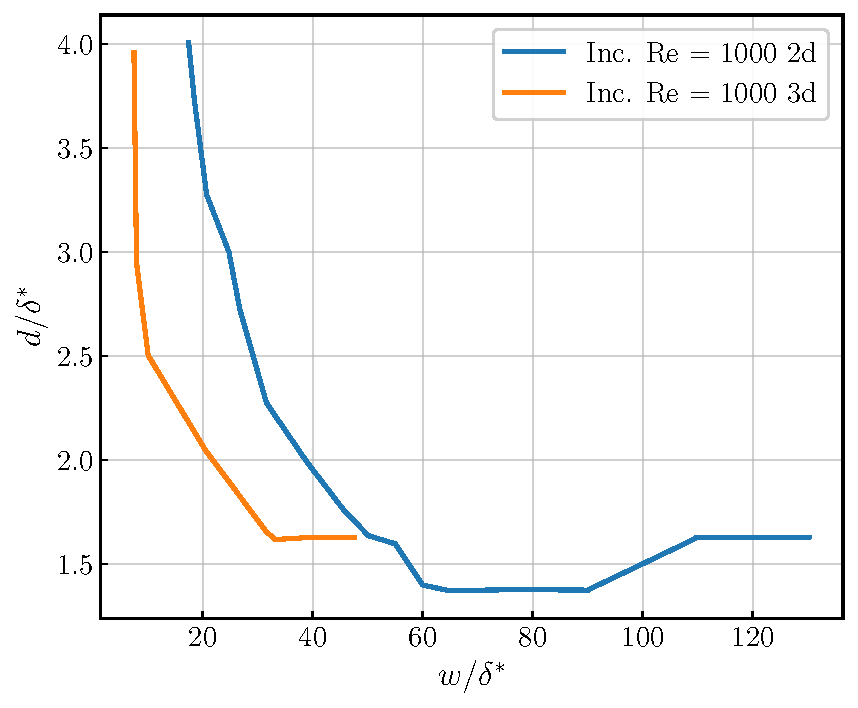
\includegraphics[width=0.5\linewidth]{Images/stabilityCurvesCombined.pdf}
  
\end{frame}

\begin{frame}
	\frametitle{3d instability (in 2d stable regime, $d=4$ $w=10$)}
	\begin{itemize}
		\item 3d instability is very different from 2d instability.
		\item For $d=4$, the unstable mode is fully concentrated in the gap, with very little influence in the boundary layer after the forward facing step.
		\item Frequency is an order of magnitude lower than the 2d instability: 
			
			$\omega_{w=\text{hopf 2d}}^{d=4} \approx 0.252\qquad\omega_{w=\text{hopf 3d}}^{d=4} \approx 0.0136$.
	\end{itemize}
	\begin{columns}[T] % [T] ensures correct vertical alignment
		\begin{column}{0.39\linewidth} % Left column
			\vspace{1.5cm}
			Time series of $v$ and $w$ \textcolor{cyan!70!black}{inside the gap} and  \textcolor{orange}{in the BL just after the gap}
		\end{column}
		\begin{column}{0.6\linewidth} % Left column
			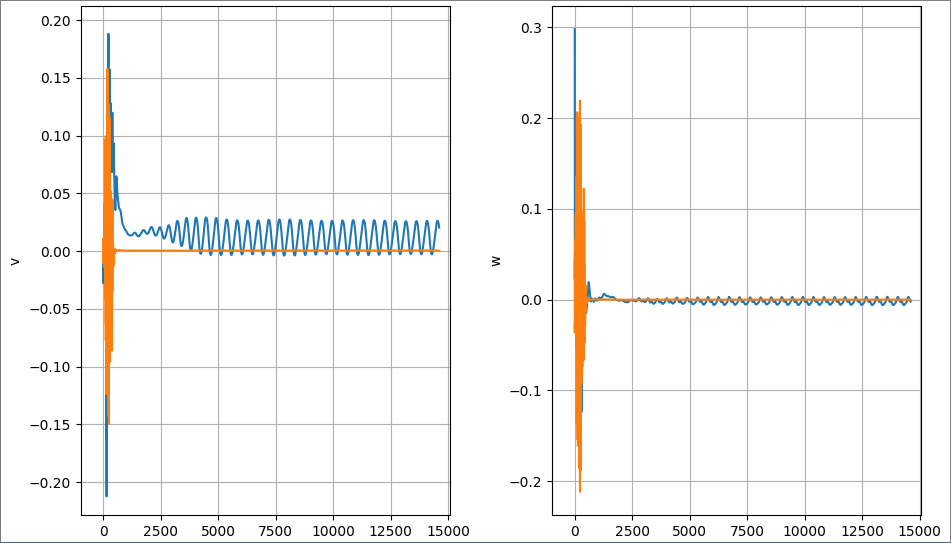
\includegraphics[width=\linewidth]{Images/d4w10_timeseries_vw.png}
		\end{column}
	\end{columns}
\end{frame}
\begin{frame}
	\begin{columns}[T] % [T] ensures correct vertical alignment
		\begin{column}{0.49\linewidth} % Left column
			$v$ at $t=t_1$ (top) and $t=t_2$ (bottom)

			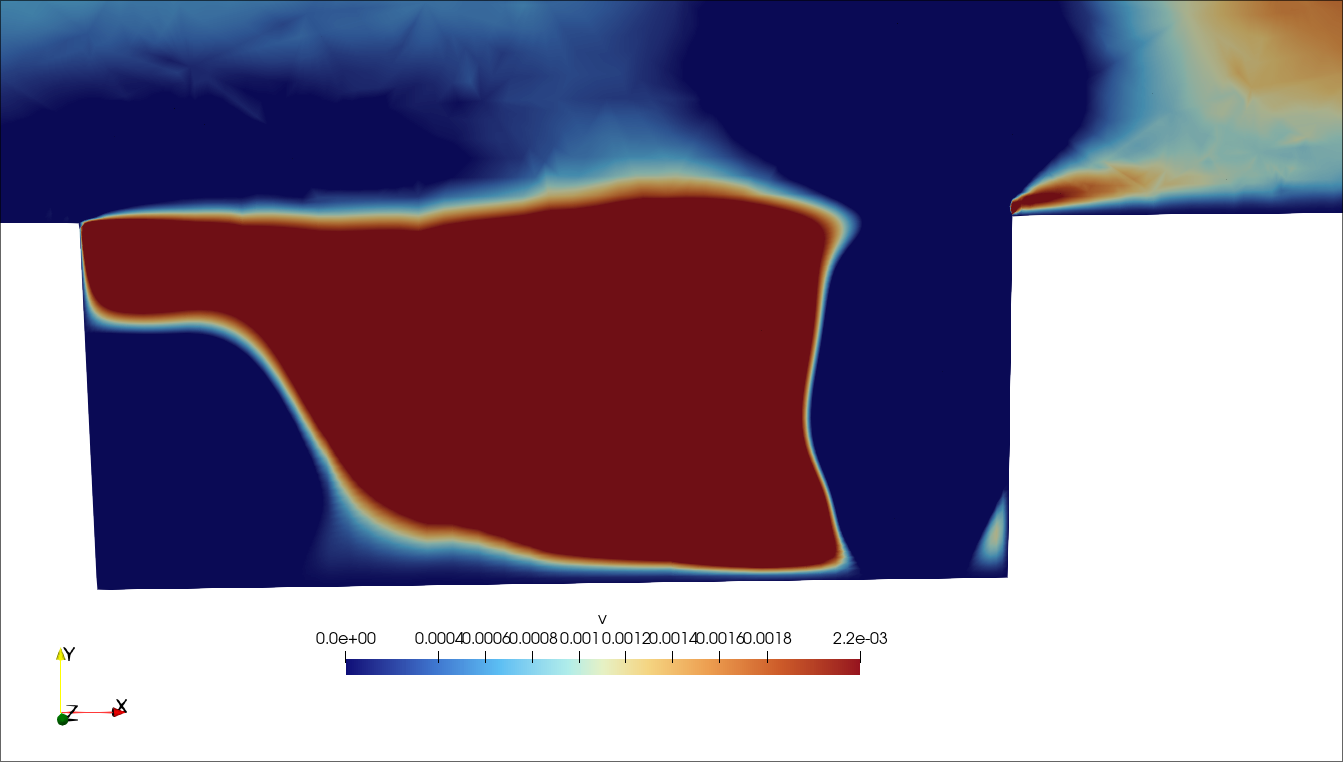
\includegraphics[width=\linewidth]{Images/d4w10_1_v.png}

			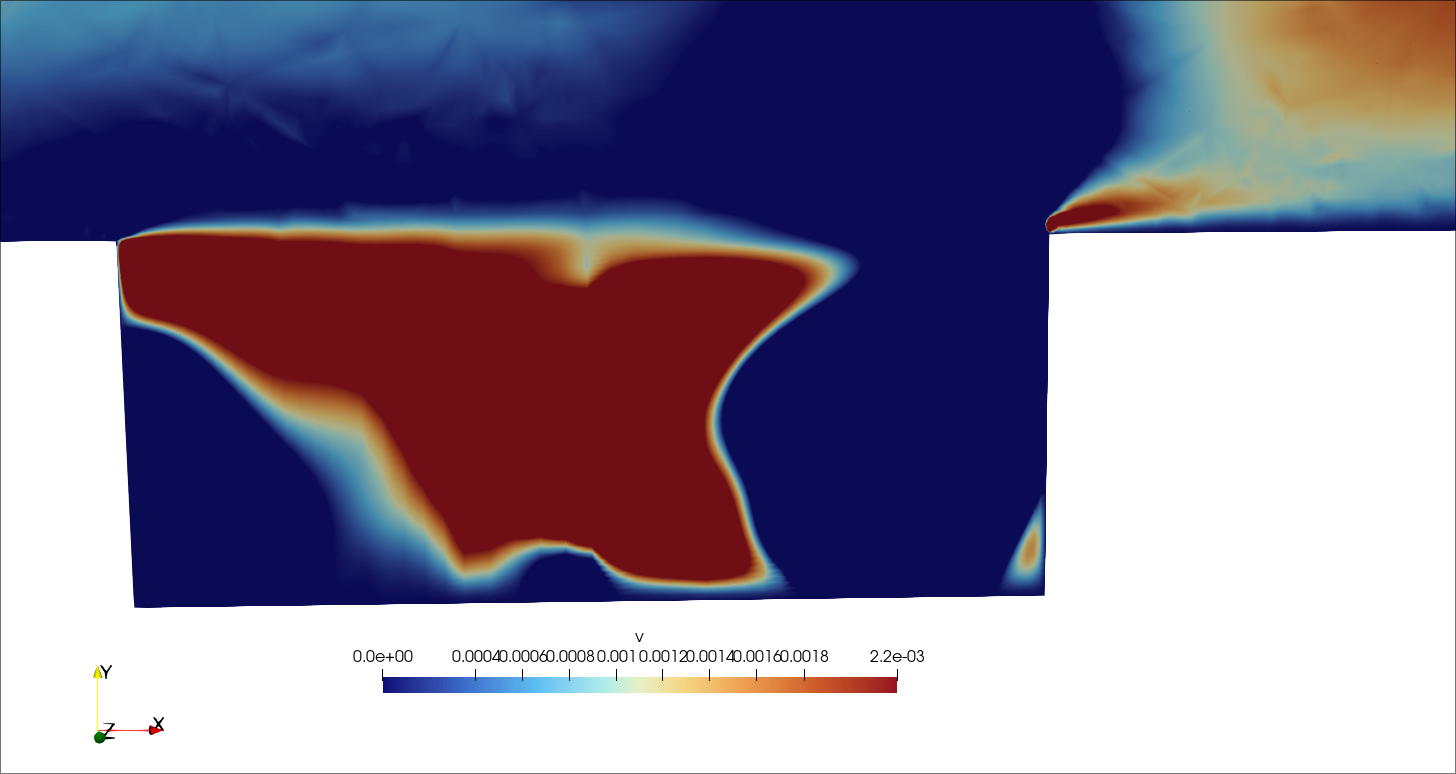
\includegraphics[width=\linewidth]{Images/d4w10_2_v.png}
		\end{column}
		\begin{column}{0.49\linewidth} % Left column
			$w$ at $t=t_1$ (top) and $t=t_2$ (bottom)

			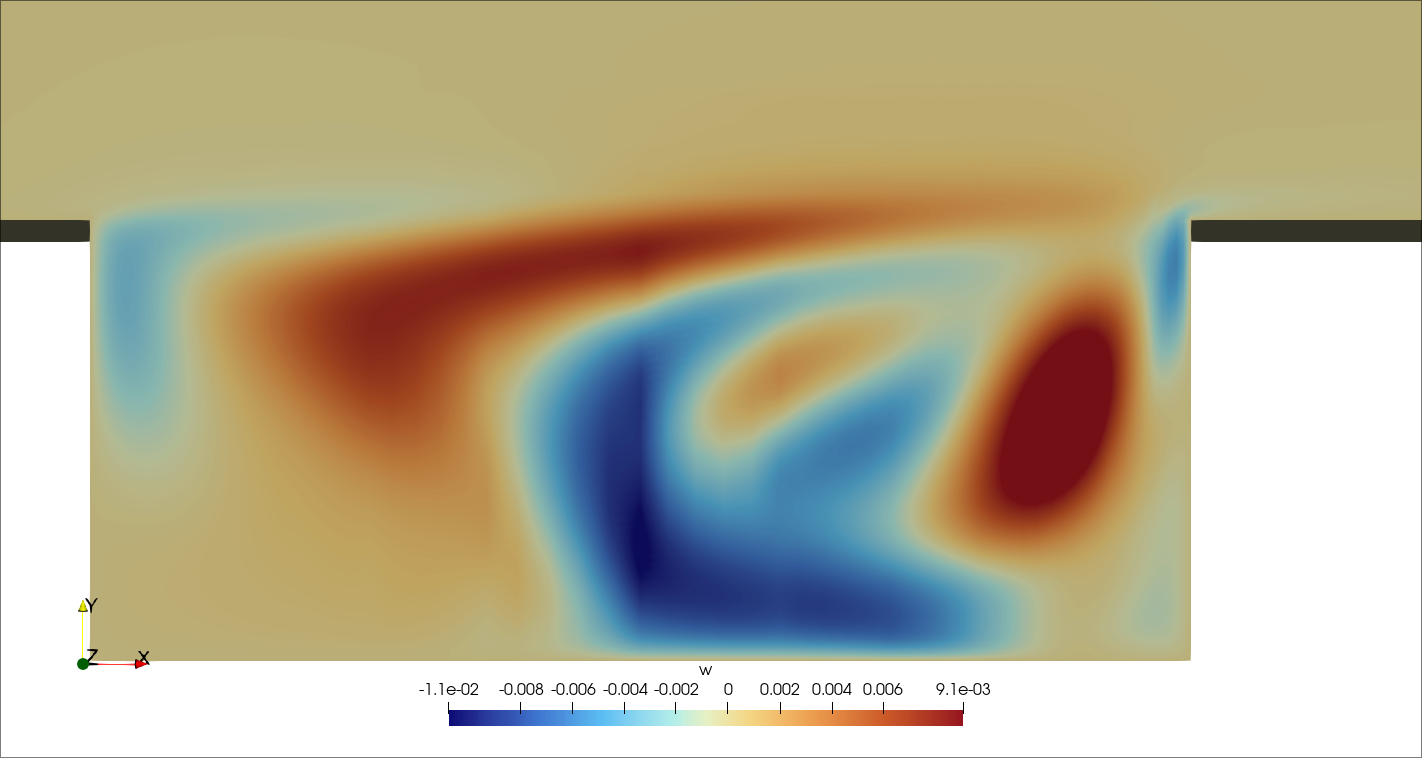
\includegraphics[width=\linewidth]{Images/d4w10_1_w.png}

			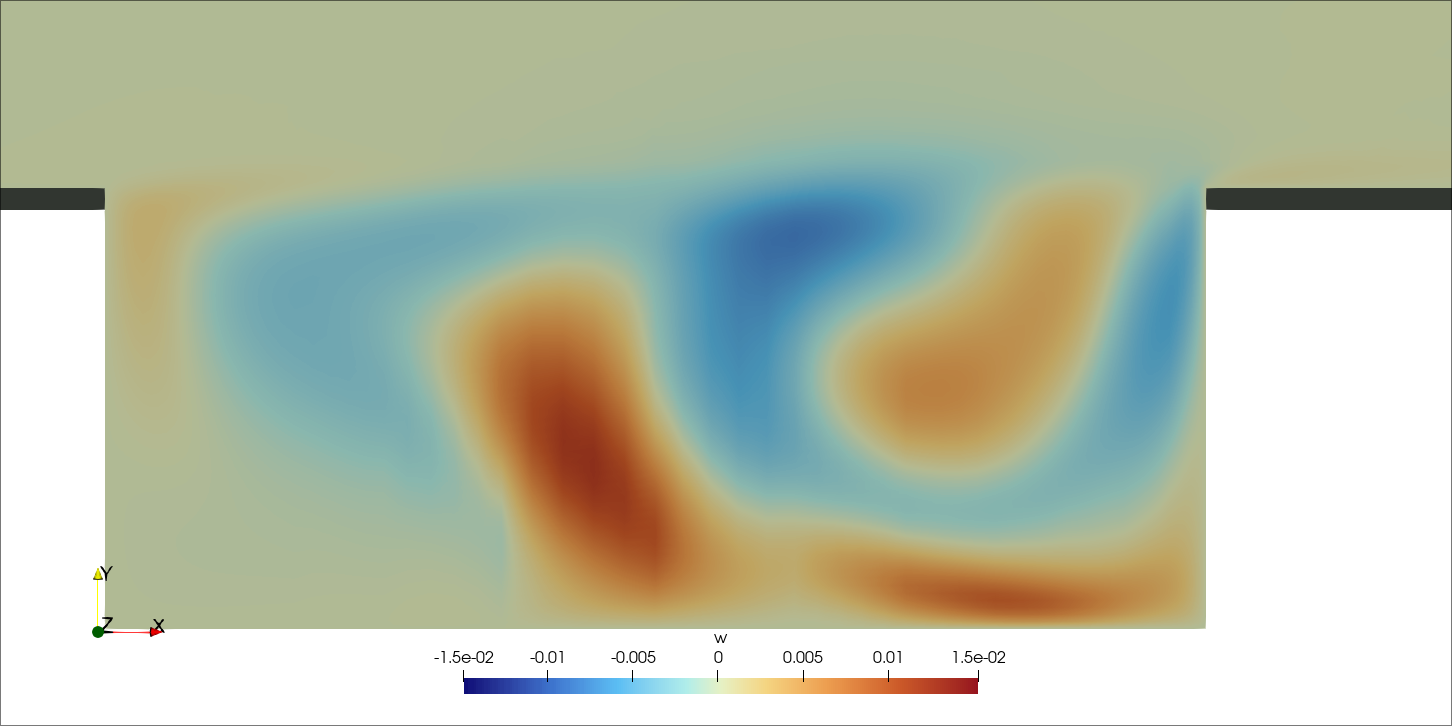
\includegraphics[width=\linewidth]{Images/d4w10_2_w.png}
		\end{column}
	\end{columns}
\end{frame}
\begin{frame}
\frametitle{2d and 3d instabilities coexisting ($d=4$ $w=18$)}
	\begin{columns}[T] % [T] ensures correct vertical alignment
		\begin{column}{0.29\linewidth} % Left column
			\begin{itemize}
				\item Time series of two points \textcolor{cyan!70!black}{inside the gap} and \textcolor{orange}{in the BL just after the gap} show the coexistence of the 2d and 3d instabilities. \item The 2d instability is only dominant in the BL, not in the cavity.
			\end{itemize}
		\end{column}
		\begin{column}{0.69\linewidth} % Left column
			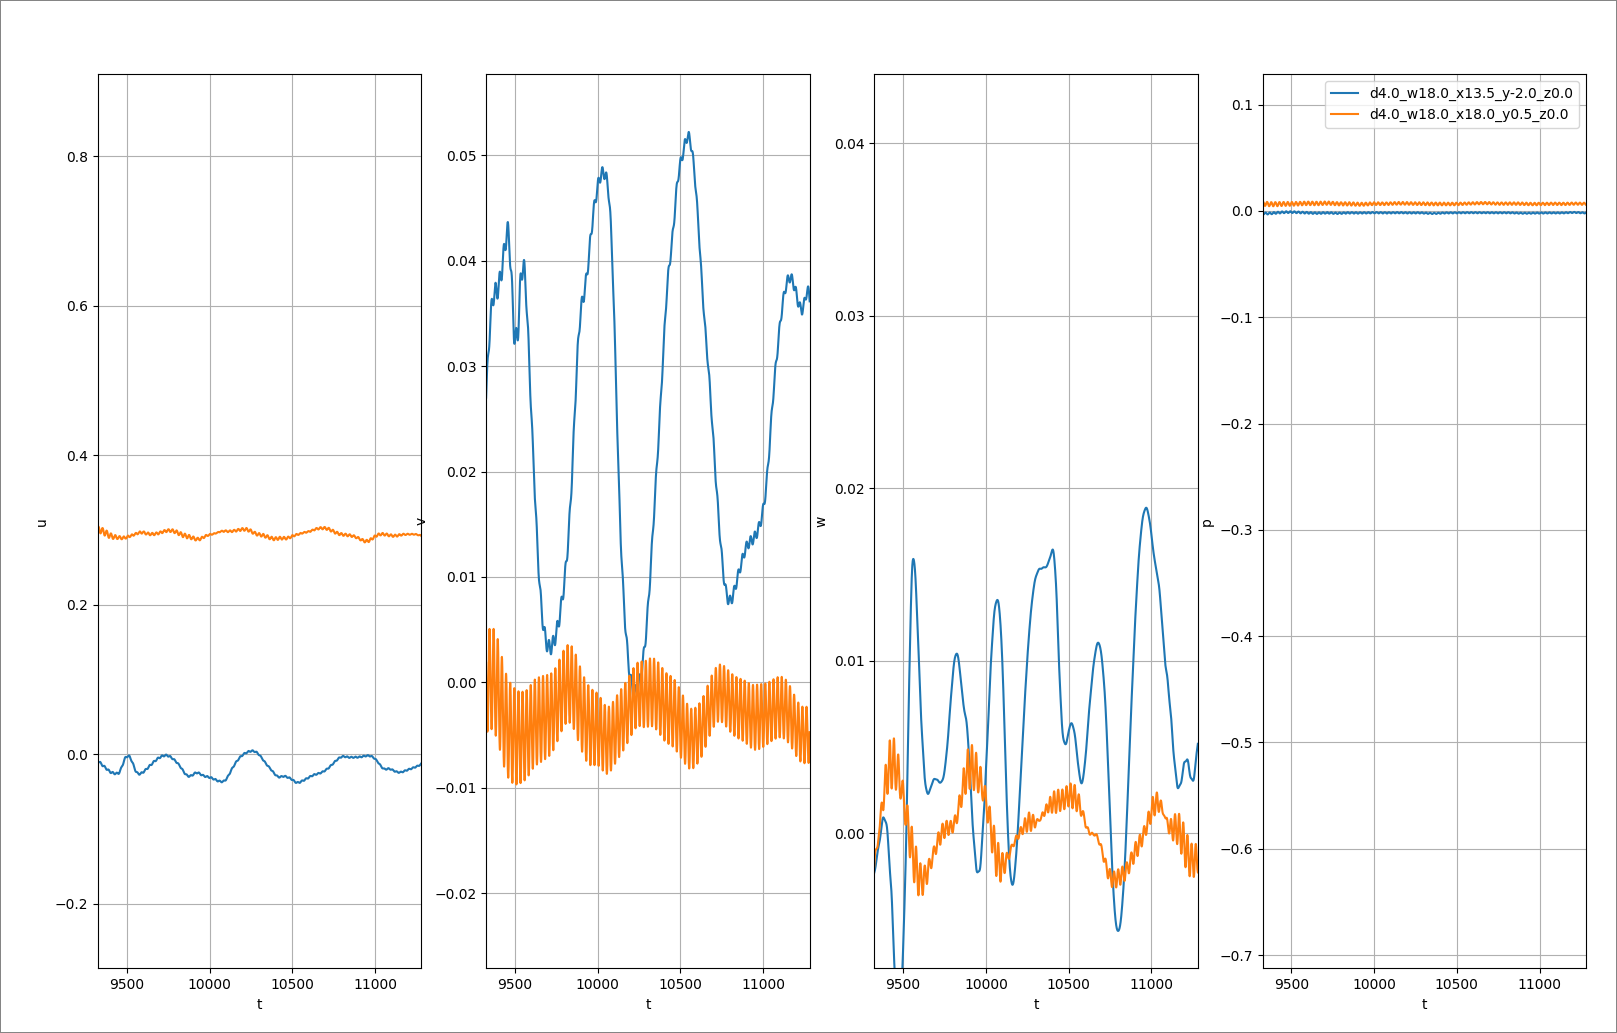
\includegraphics[width=\linewidth]{Images/d4_w18_timeseries.png}
		\end{column}
	\end{columns}
\end{frame}
\begin{frame}
  \frametitle{2d unstable and 3d stable ($d=1.5$ $w=50,80$)}

	\begin{itemize}
	  \item 3d simulations tend to the 2d unstable mode.
	  \item $\omega_{d=1.5,w=60}^{3d} = 0.142124$
	  \item $\omega_{d=1.5,w=60}^{2d} = 0.1435$
	\end{itemize}
  
\end{frame}

\begin{frame}
  \frametitle{transition at the gap, $d=1.75$, $w=80$}
  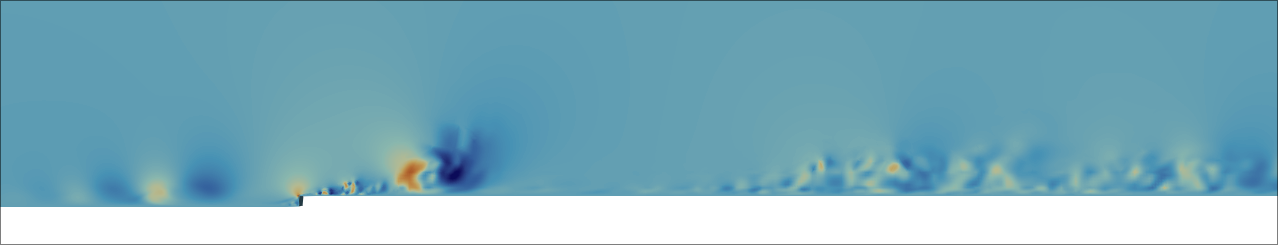
\includegraphics[width=0.8\linewidth]{Images/d1.75_w80.png}
\end{frame}

\end{document}
